%=========================================================================
% LaTeX Document
%=========================================================================

\documentclass{cbxposter}

% Automatix LaTeX build system modules

\usepackage{svg}

%-------------------------------------------------------------------------
% Setup
%-------------------------------------------------------------------------

\title
{%
  Panorama: Integrated Rack-Scale Acceleration for Computational Pangenomics
}

\authors
{%
  Nicholas Cebry\\
  Prof. Christopher Batten
}

\inst
{%
  School of Electrical and Computer Engineering \\[0.12in]
  Cornell University
}

\name    {Nicholas Cebry}
%\address {323 Rhodes Hall, Ithaca, NY 14853}
%\web     {http://www.csl.cornell.edu/~cbatten}
\email   {nfc35@cornell.edu}

%-------------------------------------------------------------------------
% macros
%-------------------------------------------------------------------------

\renewcommand{\medskip}{\vspace{0.5in}}
\renewcommand{\smallskip}{\vspace{0.16667in}}

%-------------------------------------------------------------------------
% Begin Document
%-------------------------------------------------------------------------

\begin{document}
\begin{frame}[fragile,t]{}
\vspace{0.1in}
\begin{columns}[T]

%=========================================================================
% Column 1
%=========================================================================

\begin{column}{10.5in}
\vspace{0.4in}

%-------------------------------------------------------------------------
% Abstract
%-------------------------------------------------------------------------

\begin{block}{Project overview}
  \begin{center}
    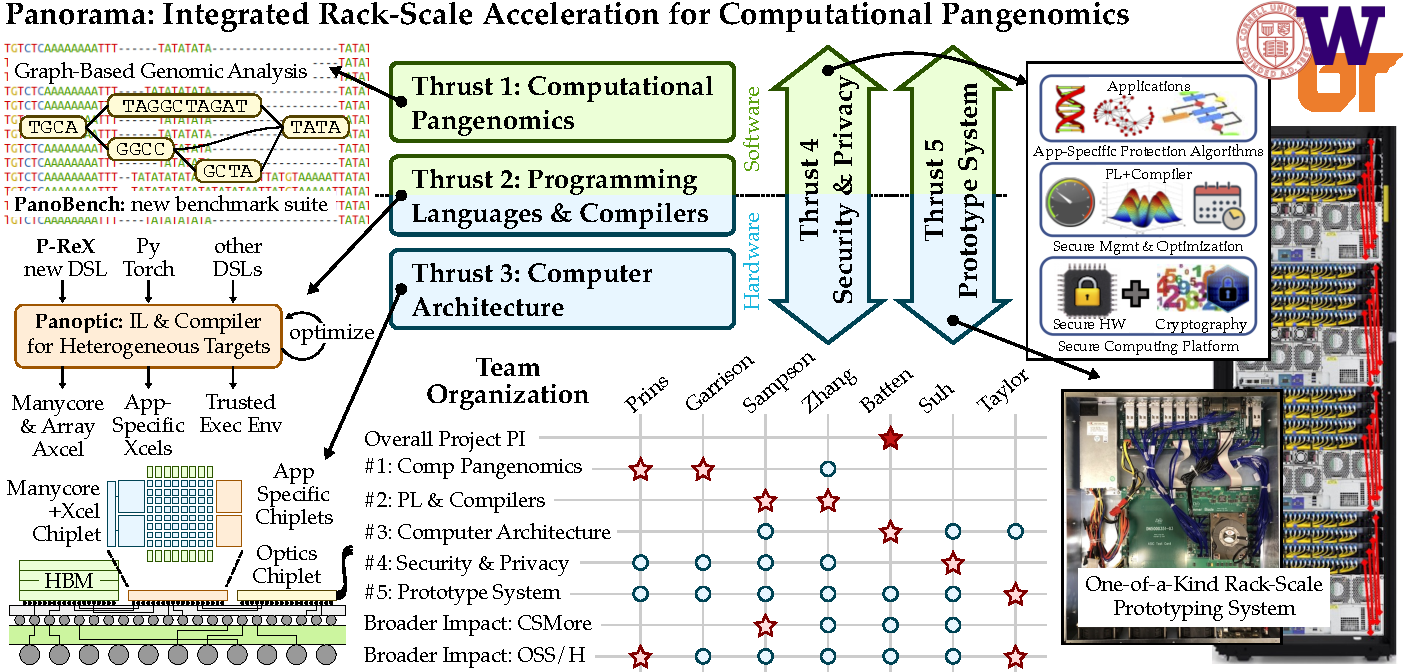
\includegraphics[width=0.95\tw]{overview.pdf}
  \end{center}

  \smallskip

  The Panorama project is a collaborative effort between seven professors
  at three different universities performing cross-stack acceleration of
  pangenomic computation. Research is occurring in five main thrusts: 1)
  new algorithms for pangenomics 2) programming languages and compilers to
  make it easier for bioinformaticists to write performant code 3)
  specialized computer architectures for faster processing of pangenomic
  workloads 4) cryptography for secure and private processing of pangenomic
  data 5) development of a prototype rack-scale processing system.

  \begin{center}
  \begin{minipage}[t]{0.135\tw}
    \vspace{0pt}\centering
    \smallskip
    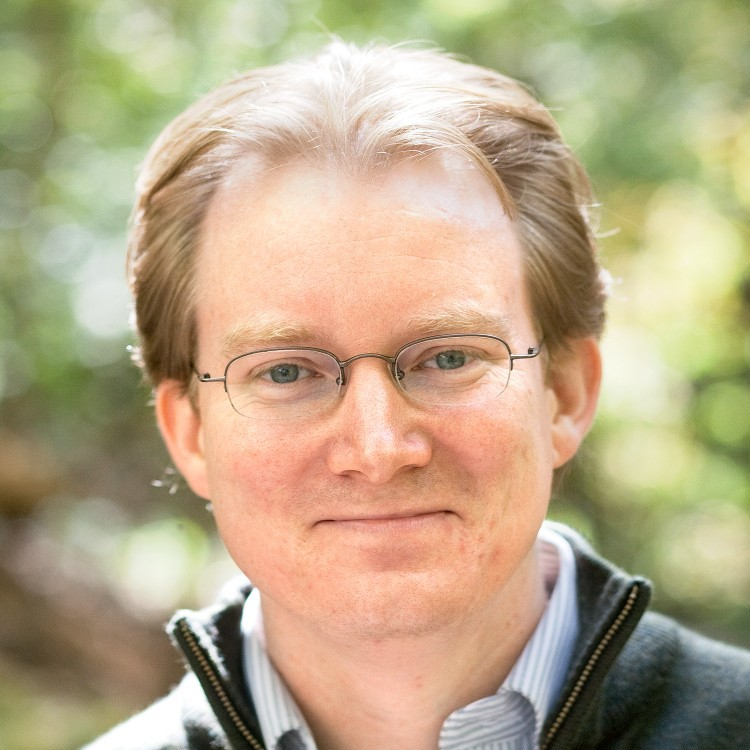
\includegraphics[width=\tw]{batten2.jpg}\\
    \smallskip
    Christopher Batten\\[0.005in]
    Cornell
  \end{minipage}
  \begin{minipage}[t]{0.135\tw}
    \vspace{0pt}\centering
    \smallskip
    
\includegraphics[width=\tw]{garrison2.jpg}\\
    \smallskip
    Erik Garrison\\
    Tennessee
  \end{minipage}
  \begin{minipage}[t]{0.135\tw}
    \vspace{0pt}\centering
    \smallskip
    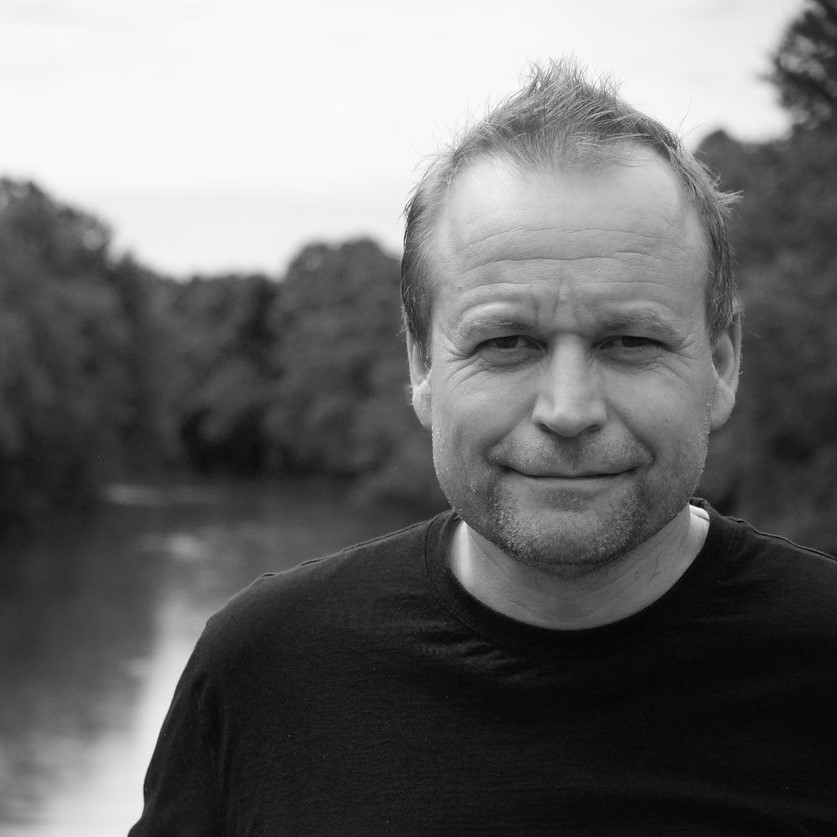
\includegraphics[width=\tw]{prins3.jpg}\\
    \smallskip
    Pjotr Prins\\
    Tennessee
  \end{minipage}
  \begin{minipage}[t]{0.135\tw}
    \vspace{0pt}\centering
    \smallskip
    
\includegraphics[width=\tw]{sampson2.jpg}\\
    \smallskip
    Adrian Sampson\\
    Cornell
  \end{minipage}
  \begin{minipage}[t]{0.135\tw}
    \vspace{0pt}\centering
    \smallskip
    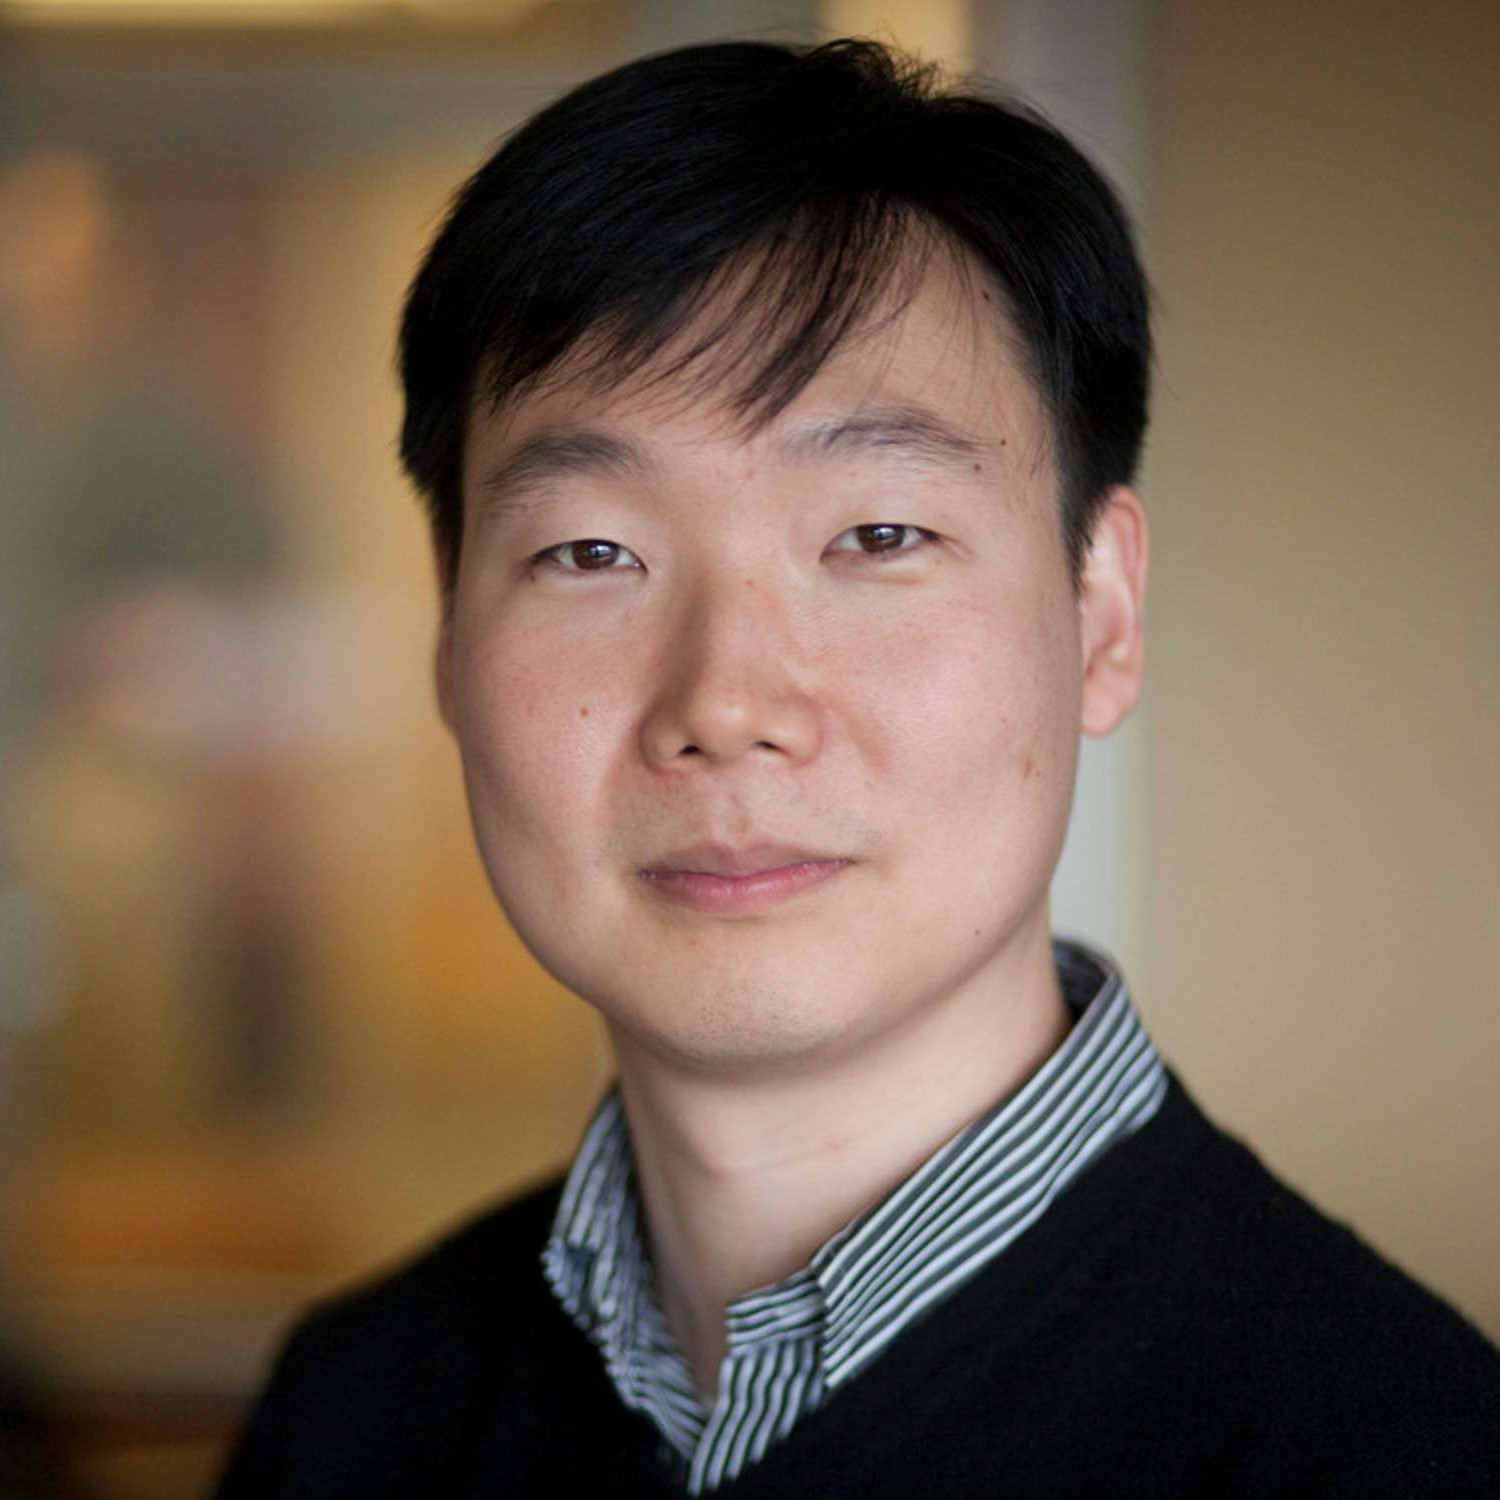
\includegraphics[width=\tw]{suh2.jpg}\\
    \smallskip
    Edward Suh\\
    Cornell
  \end{minipage}
  \begin{minipage}[t]{0.135\tw}
    \vspace{0pt}\centering
    \smallskip
    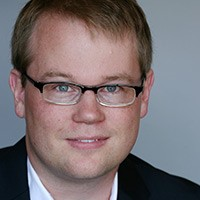
\includegraphics[width=\tw]{taylor2.jpg}\\
    \smallskip
    Michael Taylor\\
    Washington
  \end{minipage}
  \begin{minipage}[t]{0.135\tw}
    \vspace{0pt}\centering
    \smallskip
    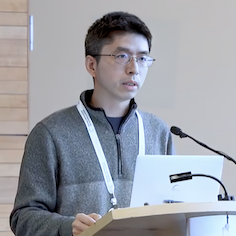
\includegraphics[width=\tw]{zhang2.png}\\
    \smallskip
    Zhiru Zhang\\
    Cornell
  \end{minipage}
\end{center}
\end{block}

%-------------------------------------------------------------------------
% Pangenomics
%-------------------------------------------------------------------------

\vspace{0.67in}
\begin{block}{Pangenomics}
  \begin{center}
    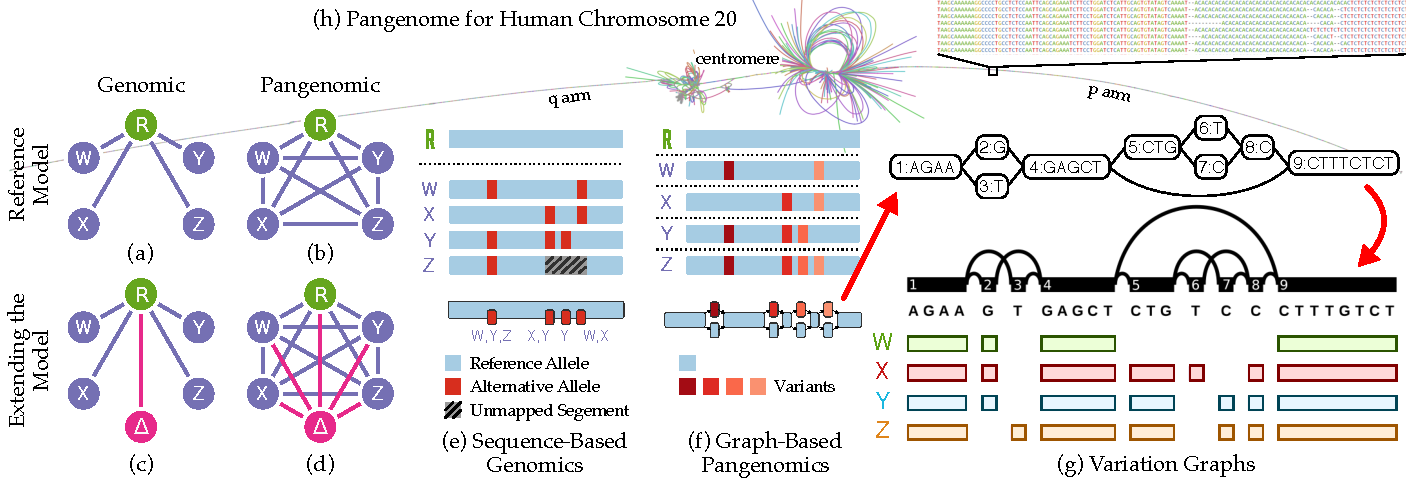
\includegraphics[width=0.95\tw]{pangenomics.pdf}
  \end{center}

  Adapted from: https://www.ncbi.nlm.nih.gov/pmc/articles/PMC8006571

  \smallskip

  Pangenomics refers to the use of graphs for the analysis of genomic data
  instead of the linear structures used in traditional genomics. While
  regular genomics relies on one-to-one comparisons between the genome being
  studied and a single reference genome, pangenomics utilizes all-to-all
  comparisons between the genome being studied and a population of reference
  genomes to provide additional insight.
  
\end{block}

\end{column}

\begin{column}{10.5in}
  \vspace{0.4in}

  \begin{block}{Collaborators: Accelerating Visualization}
    \smallskip
    Jiajie Li and Niklas Schmelzle from Prof. Zhang's group have vorked on
    accelerating the algorithm for display of pangenome graphs through
    improved hardware-aware programming and use of GPUs.
    \begin{center}
      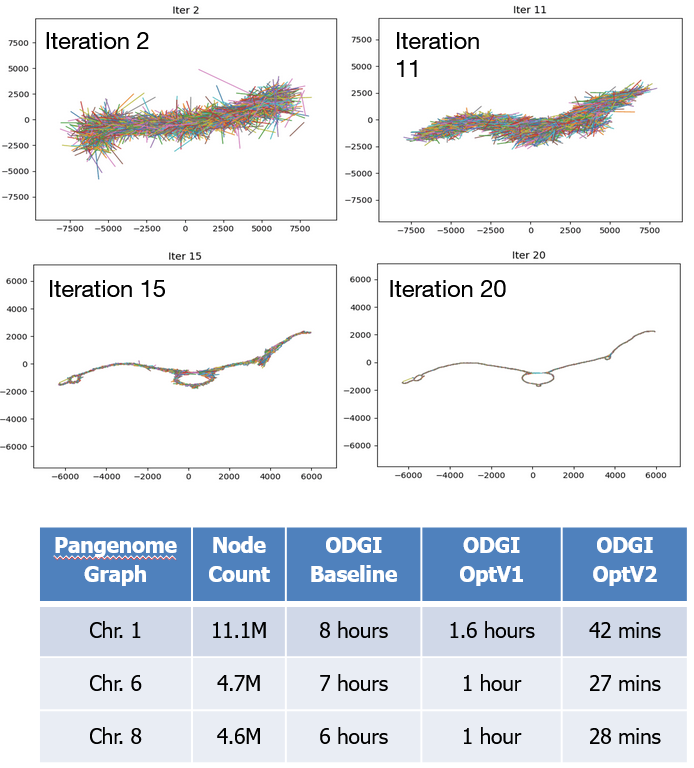
\includegraphics[width=0.95\tw]{accelerate-odgi.png}
    \end{center}
  \end{block}

\vspace{0.67in}
\begin{block}{Collaborators: Protecting Privacy}
    \smallskip
    Pengzhi Huang and Muhammad Umar from Prof. Suh's group have explored
    ways to protect individual privacy while performing computation on data
    spanning large populations through cryptography and generative AI.
    \begin{center}
      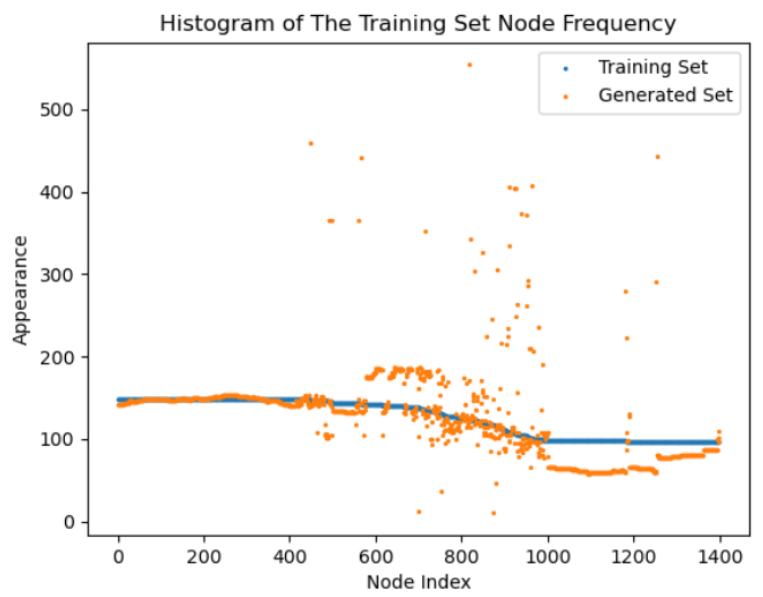
\includegraphics[width=0.95\tw]{generated-genome.png}
    \end{center}
  \end{block}

\end{column}

%=========================================================================
% Column 2
%=========================================================================

\begin{column}{10.5in}
\vspace{0.4in}

%-------------------------------------------------------------------------
% Approach
%-------------------------------------------------------------------------

\begin{block}{Gap-Affine Alignment}
  \smallskip

  One important step in the genomics pipeline is read alignment. When an
  organism's genome is read, the process produces a number of randomly
  selected subsequences of their genome, known as reads. In order to
  evaluate the genome, these reads must be assembled into the complete
  genome. This is typically done by comparing each read to an already
  assembled reference genome, and determining the most likely position of
  the read in the genome based on its similarity to a location in the
  reference. In classic genomics (using a linear reference), this comparison
  is often done with the Smith-Waterman dynamic programming algorithm. In
  Smith-Waterman, the section of the reference being evaluated is placed
  along the top of a matrix, and the read is placed along the left side.
  Cells of the matrix are filled out from the top left to the bottom right,
  with values dictated by scoring parameters for the various operations
  (match, insertion, deletion, substitution). Biologically, insertions and
  deletions are likely to be longer than a single base, so the Smith-Waterman
  algorithm assigns a separate gap-opening and gap extension penalty. The
  following matrix uses a match score of 3, substitution penalty of 2, gap
  opening penalty of 2, and gap extension penalty of 1.

  \begin{center}
    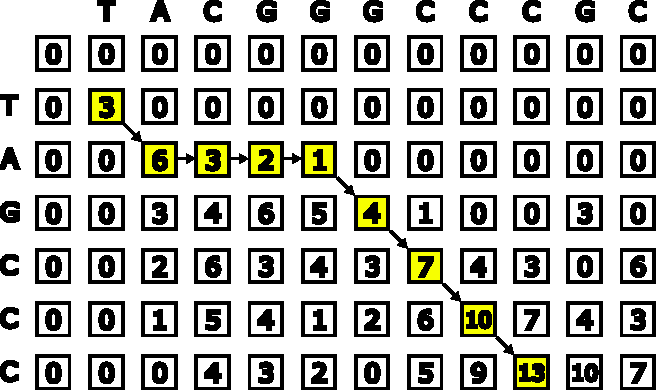
\includegraphics[width=0.95\tw]{gap-affine.pdf}
  \end{center}

\end{block}

%-------------------------------------------------------------------------
% Background
%-------------------------------------------------------------------------

\vspace{0.67in}
\begin{block}{Edit Distance Alignment}
  \smallskip

  Edit distance is another mechanism for comparing the similarity of two
  sequences. Instead of assigning separate scores to each of the different
  alignment operations like Smith-Waterman, we just ocunt the total number
  of non-match operations. It can be thought of like a special case of the
  Smith-Waterman algorithm. The following matrix uses edit distance to
  perform the same alignment as the gap-affine matrix above. This is
  equivalent to a Smith-Waterman scoring scheme of match score 0,
  substitution penalty 1, gap opening penalty of 0, and gap extension
  penalty of 1.

  \begin{center}
    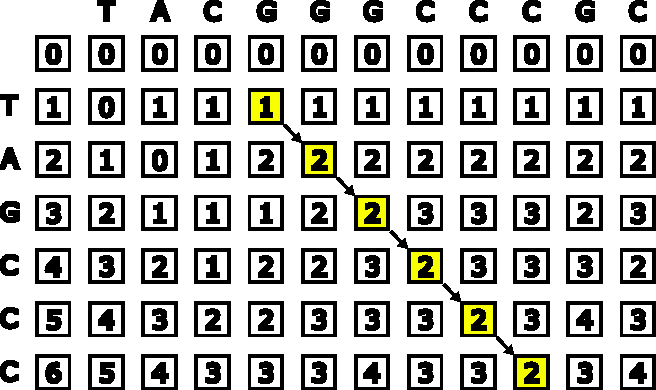
\includegraphics[width=0.95\tw]{edit-dist.pdf}
  \end{center}

  While edit distance is less flexible than Smith-Waterman, it is much more
  ammenable to acceleration, and often produces substantially similar results.
  And for instances where the flexibility of Smith-Waterman is necessary, edit
  distance can serve as a filtering mechanism to eliminate less-promising
  alignments before performing the more computationally expensive Smith-Waterman
  algorithm.

\end{block}

\end{column}

%=========================================================================
% Column 3
%=========================================================================

\begin{column}{10.5in}
\vspace{0.4in}

%-------------------------------------------------------------------------
% RPDN
%-------------------------------------------------------------------------

\begin{block}{Related work: SeGraM}
  \smallskip

  One recently published work called SeGraM accelerates the bitap algorithm
  for compuation of edit distance. Bitap is an automata-based algorithm which
  uses a single computer word to represent state as it searches for matches
  between the read and reference. To support non-exact matches, it keeps a
  separate state vector for each potential number of edits being considered.
  Segram uses a systolic array to compute the states for each edit distance
  at each reference character.

  \begin{minipage}[t]{0.45\tw}
    \vspace{0pt}\centering
    \smallskip
    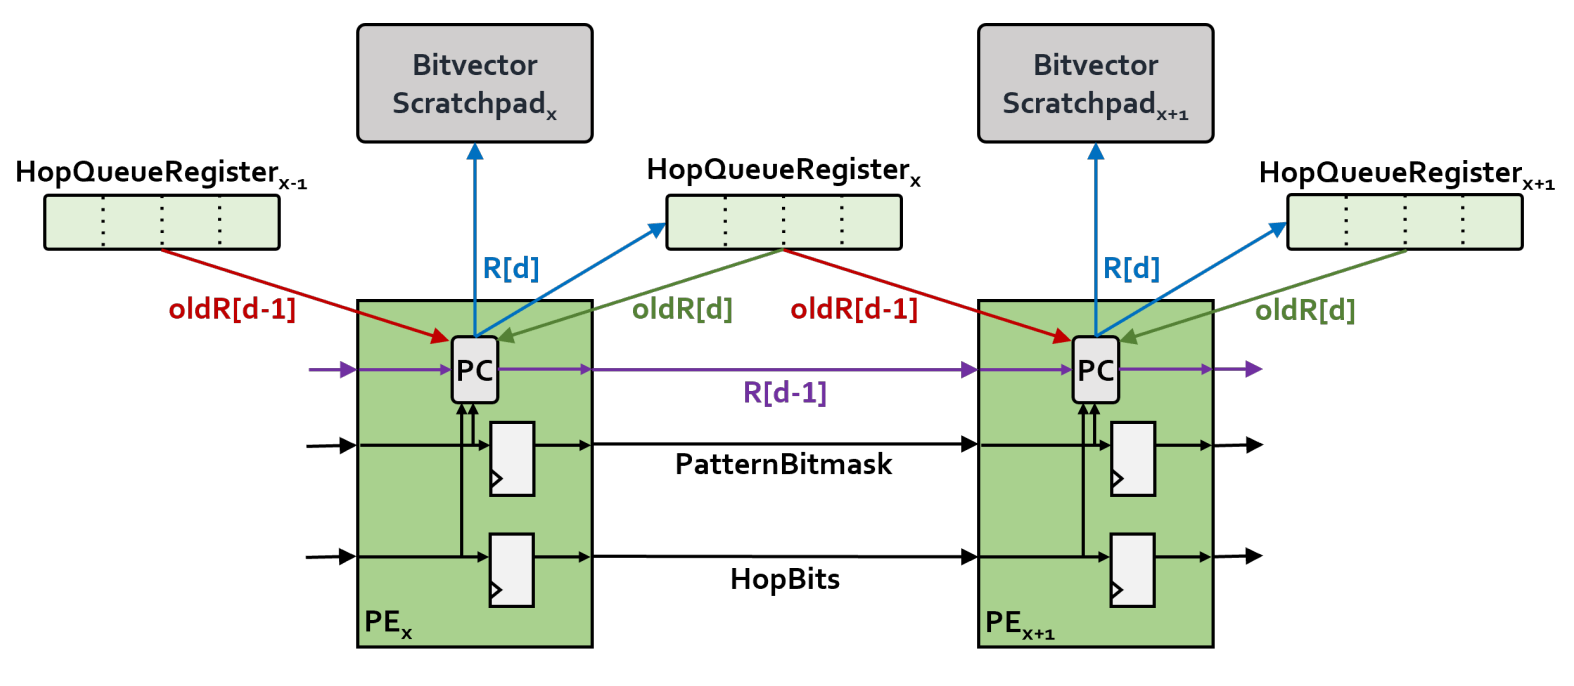
\includegraphics[width=\tw]{segram-design.png}
    \smallskip
  \end{minipage}
  \begin{minipage}[t]{0.45\tw}
    \vspace{0pt}\centering
    \smallskip
    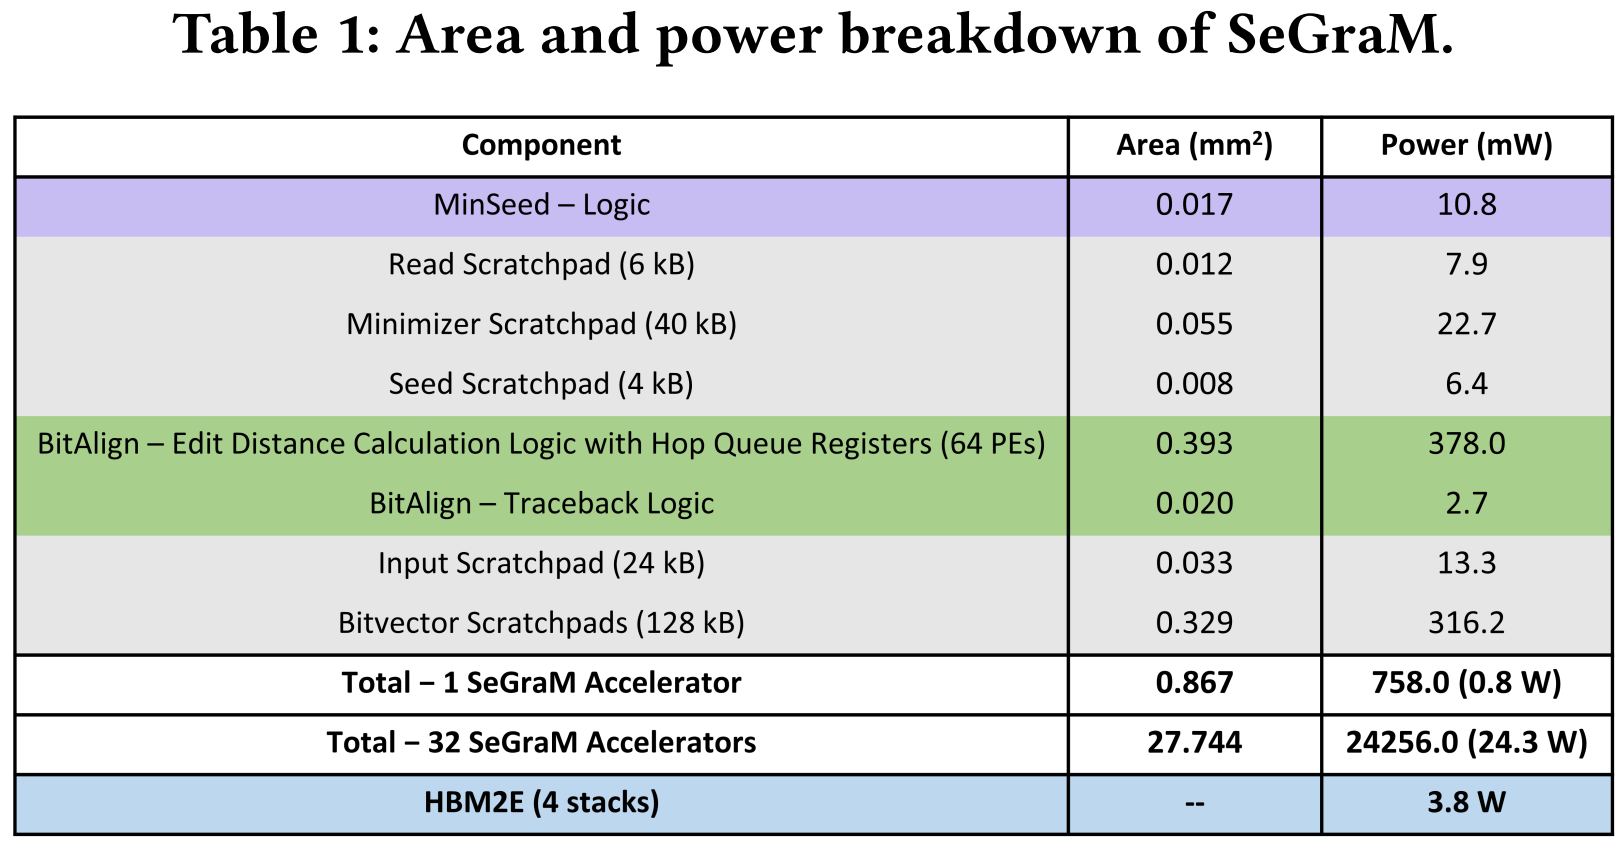
\includegraphics[width=\tw]{segram-area.png}
    \smallskip
  \end{minipage}

  source: Damla Senol Cali, et. al. 2022. SeGraM: a universal hardware
  accelerator for genomic sequence-to-graph and sequence-to-sequence 
  mapping. In Proceedings of the 49th Annual International Symposium on
  Computer Architecture (ISCA '22). Association for Computing Machinery,
  New York, NY, USA, 638–655. https://doi.org/10.1145/3470496.3527436

  \smallskip

  Note how the accelerator for the bitap algorithm and the storage for its
  output consumes most of the area and energy. We believe that by selecting
  a different algorithm for acceleration we can improve on both of these
  metrics.

\end{block}

\vspace{0.67in}
\begin{block}{Myers Algorithm}
  \smallskip

  Another algorithm that can be used for edit distance calculation is the
  Myers algorithm. This algorithm uses a dynamic programming matrix abstraction.
  It relies on the insight that differences between adjacent cells all come from
  the range [-1, 1]. With only three values to represent, only two bits are needed
  to represent the differences. An entire column of the matrix can be packed into
  two computer words, one word indicates when the delta is positive, and the other
  indicates when the delta is negative.

  \begin{center}
    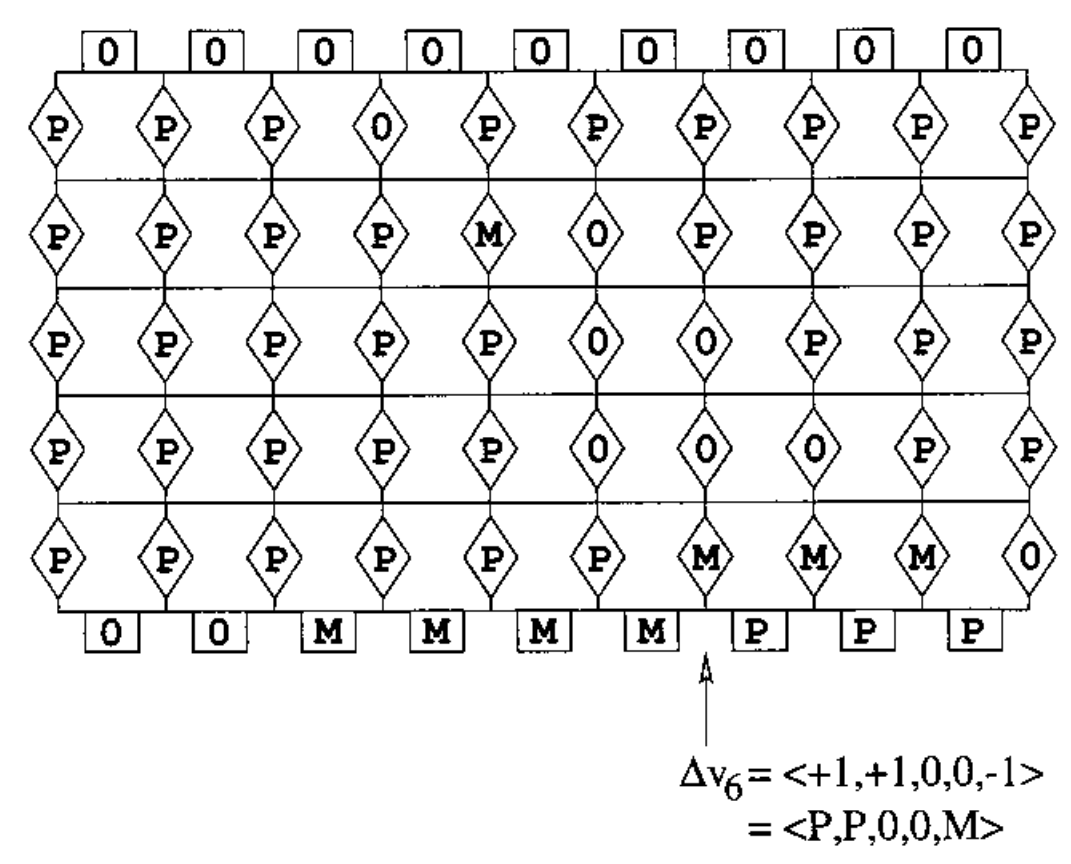
\includegraphics[width=0.75\tw]{myers-algo.png}
  \end{center}

  source: Gene Myers. 1999. A fast bit-vector algorithm for approximate string
  matching based on dynamic programming. J. ACM 46, 3 (May 1999),
  395–415. https://doi.org/10.1145/316542.316550

\end{block}

\vspace{0.67in}
\begin{block}{Myers Accelerator}
  \smallskip

  Preliminary results from using HLS to recreate a simple version of the bitap
  accelerator and compare it to a simple version of the Myers accelerator show
  promise.

  \begin{table}
  \begin{tabular}{l|r|r}
               & bitap & myers \\
    \hline
    cells      & 3988  & 2629  \\
    comb cells & 3257  & 2166  \\
    seq cells  & 705   & 437   \\
    comb area  & 3683  & 2266  \\
    total area & 6855  & 4230  \\
  \end{tabular}
  \caption{Post-synthesis area numbers for the two designs}
\end{table}

  
\end{block}

\end{column}

% %=========================================================================
% % Column 4
% %=========================================================================

% \begin{column}{10.5in}
% \vspace{0.4in}

% %-------------------------------------------------------------------------
% % Evaluation
% %-------------------------------------------------------------------------

% \begin{block}{Evaluation}
%   \centering

%   \cbxsection{Evaluation Methodology}

%   \cbxsection{Evaluation Results}

%   \smallskip\smallskip
% \end{block}

% %-------------------------------------------------------------------------
% % Acknowledgments
% %-------------------------------------------------------------------------

% \vspace{0.67in}
% \begin{block}{Acknowledgments}

%   This work was supported in part by ...

% \end{block}

% %-------------------------------------------------------------------------
% % End Document
% %-------------------------------------------------------------------------

% \end{column}
\end{columns}
\end{frame}
\end{document}

